\documentclass[12pt,a4paper]{article}
\usepackage[utf8]{inputenc}
\usepackage[T2A]{fontenc}
\usepackage[russian]{babel}
\usepackage{amsmath}
\usepackage{amsfonts}
\usepackage{amssymb}
\usepackage{graphicx}
\usepackage{geometry}
\usepackage{indentfirst}
\usepackage{multirow}
\usepackage{array}

\geometry{left=2.5cm, right=1.5cm, top=2cm, bottom=2cm}

\newcommand{\ReNum}{\mathrm{Re}}

\begin{document}


% Титульный лист
\begin{titlepage}
    \begin{center}
        % Верхняя часть с названием вуза
        \textbf{МОСКОВСКИЙ ФИЗИКО-ТЕХНИЧЕСКИЙ ИНСТИТУТ} \\
        \textbf{(НАЦИОНАЛЬНЫЙ ИССЛЕДОВАТЕЛЬСКИЙ УНИВЕРСИТЕТ)}
        \\[1cm]

        
        % Название факультета (чуть меньше)
        {\large Физтех-школа аэрокосмических технологий}
        \\[3.5cm]

        % Самое большое — полное название работы
        {\Huge \textbf{Исследование свободной турбулентной струи}}
        \\[0.5cm]

        % Блок с именами и группами (выравнивание по правому краю)
        \begin{flushright}
            \begin{tabular}{l l}
                Копышова Валентина Олеговна & Б03-304б \\
                Ларькин Глеб Сергеевич & Б03-301а \\
                Ордоньес Эррера Хулио Себастьян & Б03-304б \\
                Дай Сюй                  & Б03-304б \\
            \end{tabular}
        \end{flushright}

        \vfill

        % Нижняя часть
        {\large Долгопрудный, 2026 г.}
    \end{center}
\end{titlepage}

\tableofcontents
\newpage

\section{Цель работы}
Изучить основные закономерности поведения профиля продольной составляющей скорости для осесимметричной струи воздуха, вытекающей в неподвижное пространство. Провести измерения и построить графики, характеризующие распределение скорости в разных поперечных сечениях струи, изменение скорости на оси струи по длине, изменение полуширины струи по длине, убедиться в автомодельности полученных закономерностей.


\section{Краткие сведения о турбулентных течениях}
Из наблюдений следует, что при движении жидкости или газа можно выделить ламинарный и турбулентный режимы течения. При ламинарном движении траектории частиц, линии тока, поля скоростей и давлений имеют определенный упорядоченный характер, определяются начальными и граничными условиями к уравнениям Навье–Стокса.

Турбулентное же движение, даже при стационарных граничных условиях, является хаотическим. В нем неупорядоченно, случайно движутся и взаимодействуют между собой объемы среды (коррелированные образования, вихри или, так называемые, «моли»). Описание движения носит вероятностный, статистический характер. В теории турбулентности пока не решены вопросы возникновения турбулентного режима и получения замкнутой системы уравнений. Основным источником знаний о турбулентных течениях являются результаты экспериментальных исследований, которые, в частности, служат базой для построения приближенных полуэмпирических теорий и методов расчета.

\subsection{Схема и основные закономерности развития свободной турбулентной струи}
Одним из характерных и простых случаев распространенного турбулентного течения является струйное течение, образующееся при истечении газа или жидкости из отверстия или насадка в покоящуюся среду (так назыаемая затопленная струя)

В нашей лабораторной работе рассматривается осесимметричная струя воздуха, вытекающая из сопла диаметром $D = 60$ мм в неподвижную среду. В течении выделяют три характерные области:

\begin{figure}[h!]
\centering
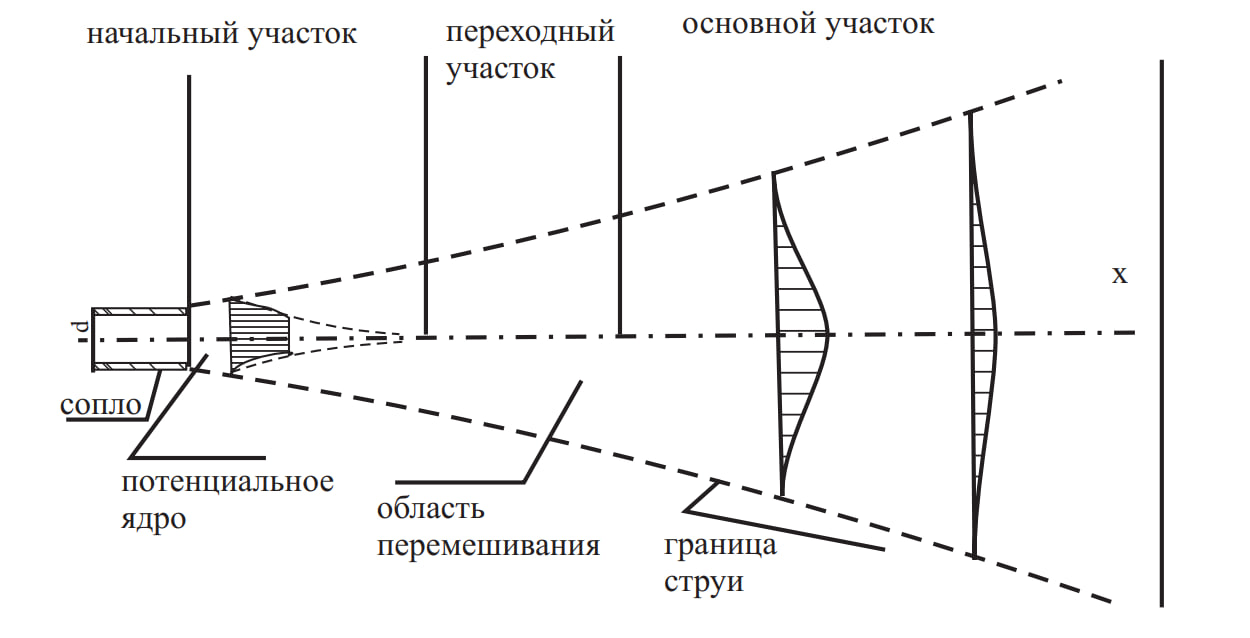
\includegraphics[width=0.7\textwidth]{photoes/scheme1.jpg}
\caption{Схема свободной затопленной турбулентной струи}
\label{fig:jet_scheme}
\end{figure}

\begin{enumerate}
    \item \textbf{Начальный участок} (вблизи среза сопла): в приосевой части сохраняется постоянная скорость $U = U_0$ (потенциальное ядро), окружённая областью перемешивания, где скорость плавно спадает до нуля.
    
    \item \textbf{Переходный участок}: область между начальным и основным участками, где потенциальное ядро исчезает.
    
    \item \textbf{Основной участок} (вдали от среза сопла): профиль скорости автомодельный, осевая скорость убывает по закону $U_{\text{ось}} \sim 1/x$, полуширина растёт линейно $r_{1/2} \sim x$.
\end{enumerate}

На границе струи происходит подсос окружающей среды за счёт турбулентного перемешивания, что приводит к росту расхода вдоль струи.

\section{Описание лабораторной установки и системы измерений}
\subsection{Установка АТМ-3}
Исследования проводятся на установке «аэродинамическая труба малая» (АТМ-3). Поток создаётся центробежным вентилятором, проходит через ресивер с выравнивающими сетками и сопло с поджатием сечения.

Установка снабжена координатником, позволяющим перемещать измерительные насадки вдоль двух взаимно перпендикулярных осей в поперечном сечении с точностью до 0,1 мм. Сам координатник передвигается пдоль оси потока по направляющим рельсам. Поля скоростей в различных поперечных сечениях струи определяются по измерениям полных давлений с помощью крестообразной гребенки насадков полного давления.

\begin{figure}[h!]
\centering
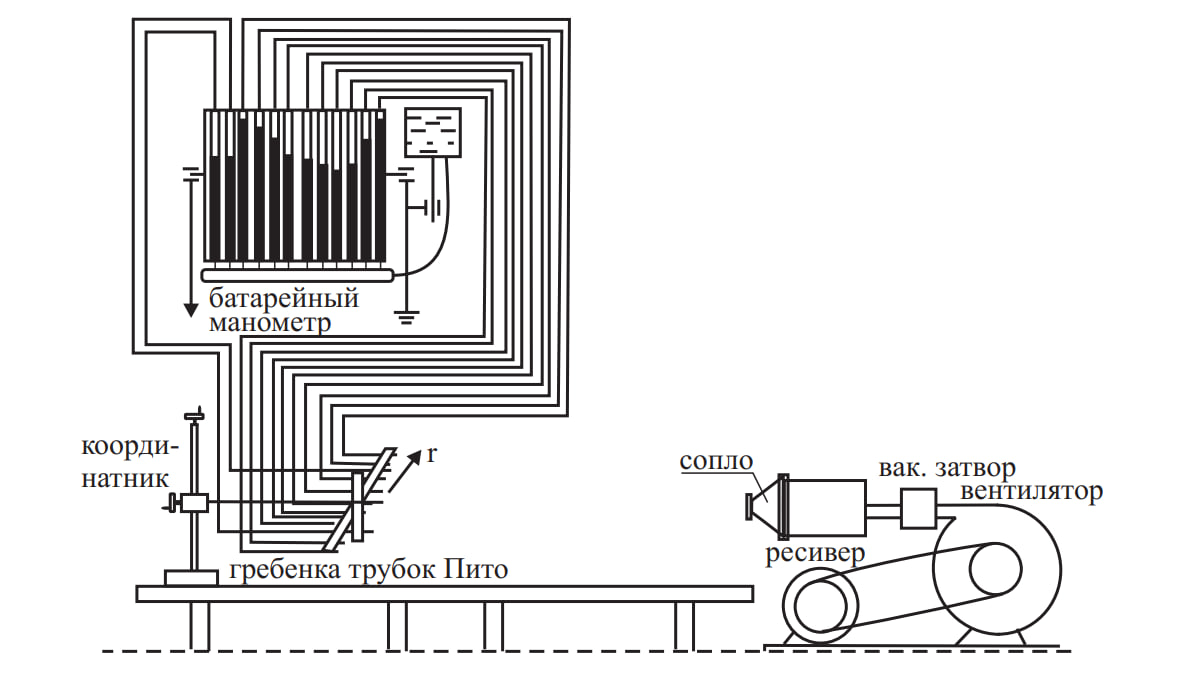
\includegraphics[width=0.5\textwidth]{photoes/scheme2.jpg}
\hfill
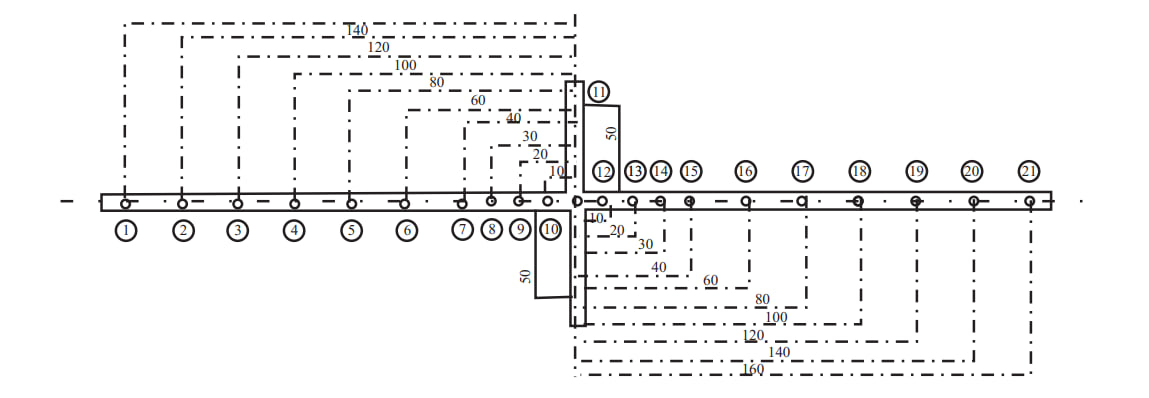
\includegraphics[width=0.5\textwidth]{photoes/scheme3.jpg}
\caption{Схема установки АТМ-3}
\label{fig:setup}
\end{figure}

\subsection{Принцип измерения скорости}
Скорость определяется по разности полного $p_0$ и статического $p$ давлений через уравнение Бернулли для несжимаемой жидкости ($M = U/a \ll 1$):
\begin{equation}
p_0 = p + \frac{\rho U^2}{2}.
\label{eq:bernoulli}
\end{equation}
Отсюда:
\begin{equation}
U = \sqrt{\frac{2(p_0 - p)}{\rho}}.
\label{eq:U_general}
\end{equation}

Полные давления измеряются крестообразной гребёнкой из 21 насадки полного давления, соединённой с батарейным наклонным манометром. С учётом угла наклона $\beta$ и плотности жидкости в манометре $\rho_1$:
\begin{equation}
p_0 - p = \rho_1 g \Delta L \sin\beta,
\end{equation}
где $\Delta L$ -- показание манометра вдоль трубки.

Подставляя в (\ref{eq:U_general}) и используя параметры стандартной атмосферы ($T_0 = 288$ К, $p_0 = 760$ мм рт.ст., $\rho_0 = 1.226$ кг/м$^3$), получаем рабочую формулу:
\begin{equation}
U = \sqrt{42.23 \left( \frac{T}{p} \right) \Delta L \sin\beta} \quad [\text{м/с}],
\label{eq:U_full}
\end{equation}
где $T$ -- температура в К, $p$ -- давление в мм рт.ст., $\Delta L$ -- в мм.

При малых отклонениях $T$ и $p$ от стандартных значений поправкой можно пренебречь:
\begin{equation}
U \approx 4 \sqrt{\Delta L \sin\beta} \quad [\text{м/с}].
\label{eq:U_simplified}
\end{equation}


\section{Ход работы}
\begin{enumerate}
    \item Ознакомились с теорией к лабораторной работе и установкой, проверили горизонтальность гребёнки и её совпадение с осью струи. Определили рабочий диапазон номеров трубок гребенки
    
    \item Включили вентилятор, дали потоку стабилизироваться.
    
    \item Зафиксировали параметры окружающей среды:
    \begin{itemize}
        \item Атмосферное давление: $p = 738$ мм рт. ст.
        \item Температура: $T = 293$ К.
    \end{itemize}
    
    \item Выбрали 8 сечений в диапазоне $(x-x_0)/D = 0 \div 15$ с шагом $\delta x/D = 2$ для первых 6 сечений. При расстояниях от 10 калибров (7, 8 сечения) брали шаг $\delta x/D = 2.5$
    
    \item В каждом сечении:
    \begin{itemize}
        \item установили гребёнку так, чтобы центральная трубка ($r=0$) совпадала с осью струи (по максимуму $\Delta L$);
        \item записали показания манометра $\Delta L_i$;
    \end{itemize}
    
    \end{enumerate}

\section{Результаты измерений и обработка данных}

В таблице~\ref{tab:raw_data} приведены результаты измерений показаний манометра $\Delta L$ (в мм вод. ст.) для всех 21 трубок гребенки в 8 сечениях. 


\begin{table}[h!]
\centering
\small
\caption{Показания манометра $\Delta L$ (мм вод. ст.) в зависимости от номера трубки и сечения}
\label{tab:raw_data}
\resizebox{\textwidth}{!}{%
\begin{tabular}{c|ccccccccccccccccccccc}
\toprule
\textbf{Сечение} & \multicolumn{21}{c}{\textbf{Номер трубки гребенки}} \\
\textbf{$(x-x_0)/D$} & 1 & 2 & 3 & 4 & 5 & 6 & 7 & 8 & 9 & 10 & 11 & 12 & 13 & 14 & 15 & 16 & 17 & 18 & 19 & 20 & 21 \\
\midrule
0 & & & & & & & & & 55 & 54 & 57 & 55 & 54 & & & & & & & & \\
2 & & & & & & & 266 & 188 & 73 & 57 & 57 & 57 & 68 & 173 & 260 & & & & & & \\
4 & & & & & & & 260 & 239 & 184 & 66 & 55 & 66 & 188 & 238 & 260 & & & & & & \\
6 & & & & 259 & 251 & 240 & 219 & 180 & 140 & 102 & 88 & 108 & 157 & 197 & 228 & 245 & 254 & 262 & & & \\
8 & & & 255 & 249 & 241 & 231 & 215 & 194 & 168 & 142 & 131 & 140 & 166 & 191 & 212 & 230 & 243 & 250 & 256 & & \\
10 & 249 & 248 & 246 & 239 & 233 & 223 & 210 & 203 & 187 & 174 & 168 & 170 & 180 & 195 & 209 & 222 & 233 & 240 & 247 & 250 & 252 \\
12.5 & 243 & 241 & 239 & 245 & 230 & 224 & 215 & 208 & 200 & 192 & 185 & 189 & 194 & 200 & 208 & 216 & 225 & 230 & 236 & 240 & 242 \\
15 & 238 & 236 & 233 & 232 & 227 & 223 & 213 & 209 & 207 & 203 & 199 & 204 & 206 & 208 & 212 & 224 & 230 & 233 & 235 & 236 & 238 \\
\bottomrule
\end{tabular}%
}
\end{table}

\subsection{Оценка числа Рейнольдса}
Перед обработкой выясним характер течения, оценив число Рейнольдса. 

Число Рейнольдса определяется как $\mathrm{Re} = \rho v d / \mu$, где $d = 0{,}06$~м~--- диаметр сопла, $v = 57$~м/с~--- скорость истечения.
Давление составляет $P = 738~\text{мм рт. ст.} = 738 \times 133{,}3 \approx 98\,400$~Па.
Плотность воздуха при температуре $T = 293$~К находится из уравнения состояния идеального газа:
\[
  \rho = \frac{P M}{R T} \approx 1{,}17~\text{кг/м}^3.
\]
Динамическая вязкость воздуха хорошо описывается степенным законом
\[
  \mu = 1{,}75 \times 10^{-5} \left(\frac{T}{273}\right)^{3/4}
       \approx 1{,}85
 \times 10^{-5}~\text{Па{\,·\,}с}.
\]
Подставляя найденные значения, получаем
\[
  \mathrm{Re} \approx 2{,}3 \times 10^{5}.
\]
Столь высокое значение числа Рейнольдса ($\mathrm{Re} \gg 2300$ - критическое трубное число Рейнольдса) свидетельствует об изначально турбулентном режиме течения.

\subsection{Обработка}


\begin{figure}[h!]
\centering
 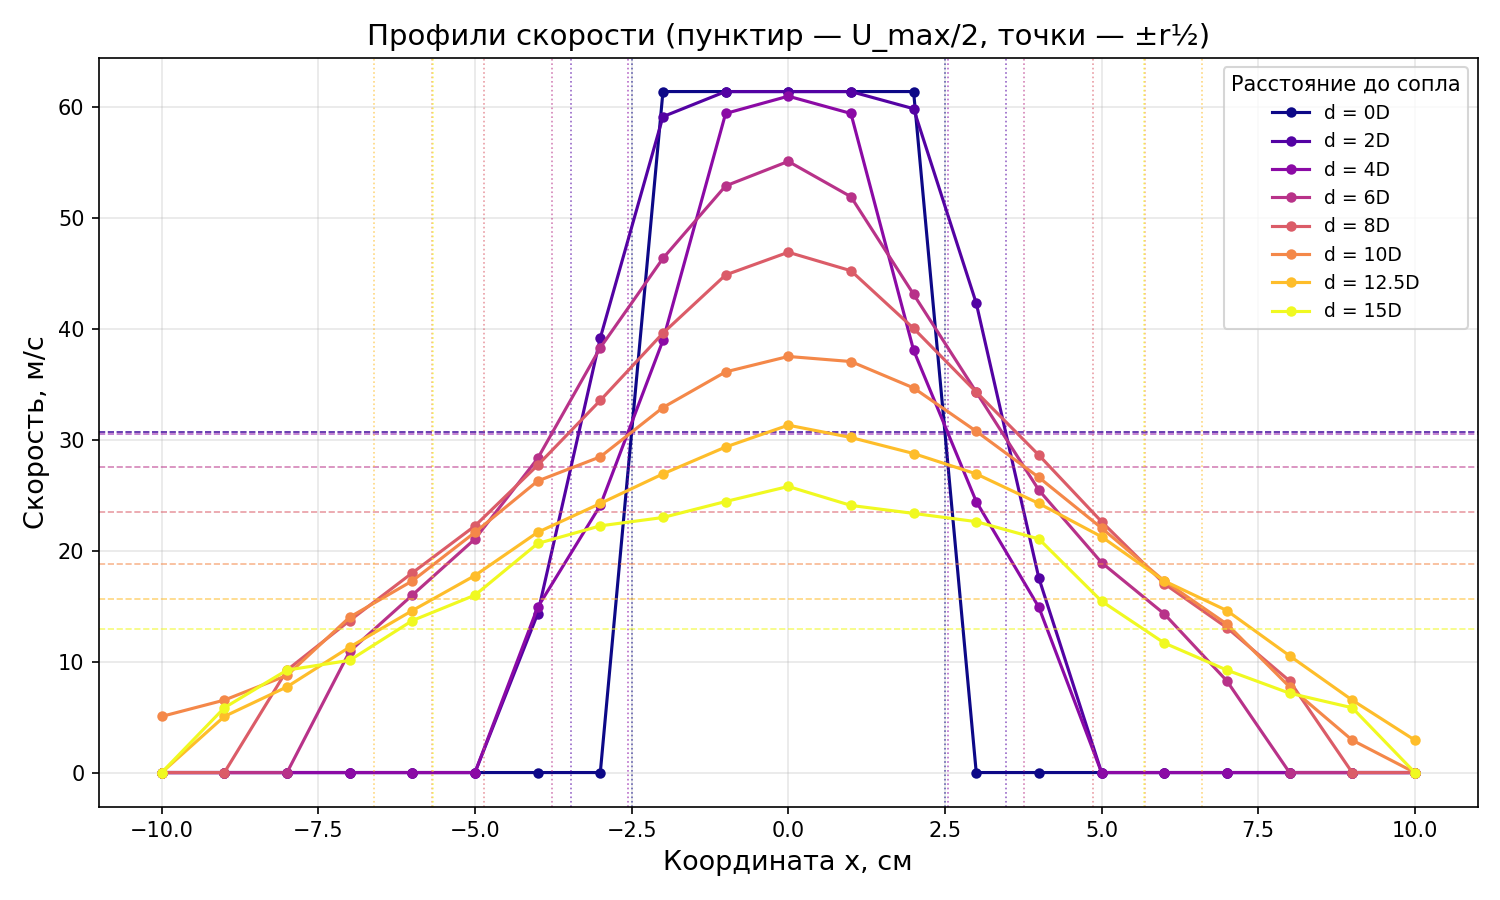
\includegraphics[width=0.75\textwidth]{photoes/velocity_profile.png}
\caption{Профили скорости $U(r)$ в различных сечениях струи}
\label{fig:velocity_profile}
\end{figure}

\begin{figure}[h!]
\centering
 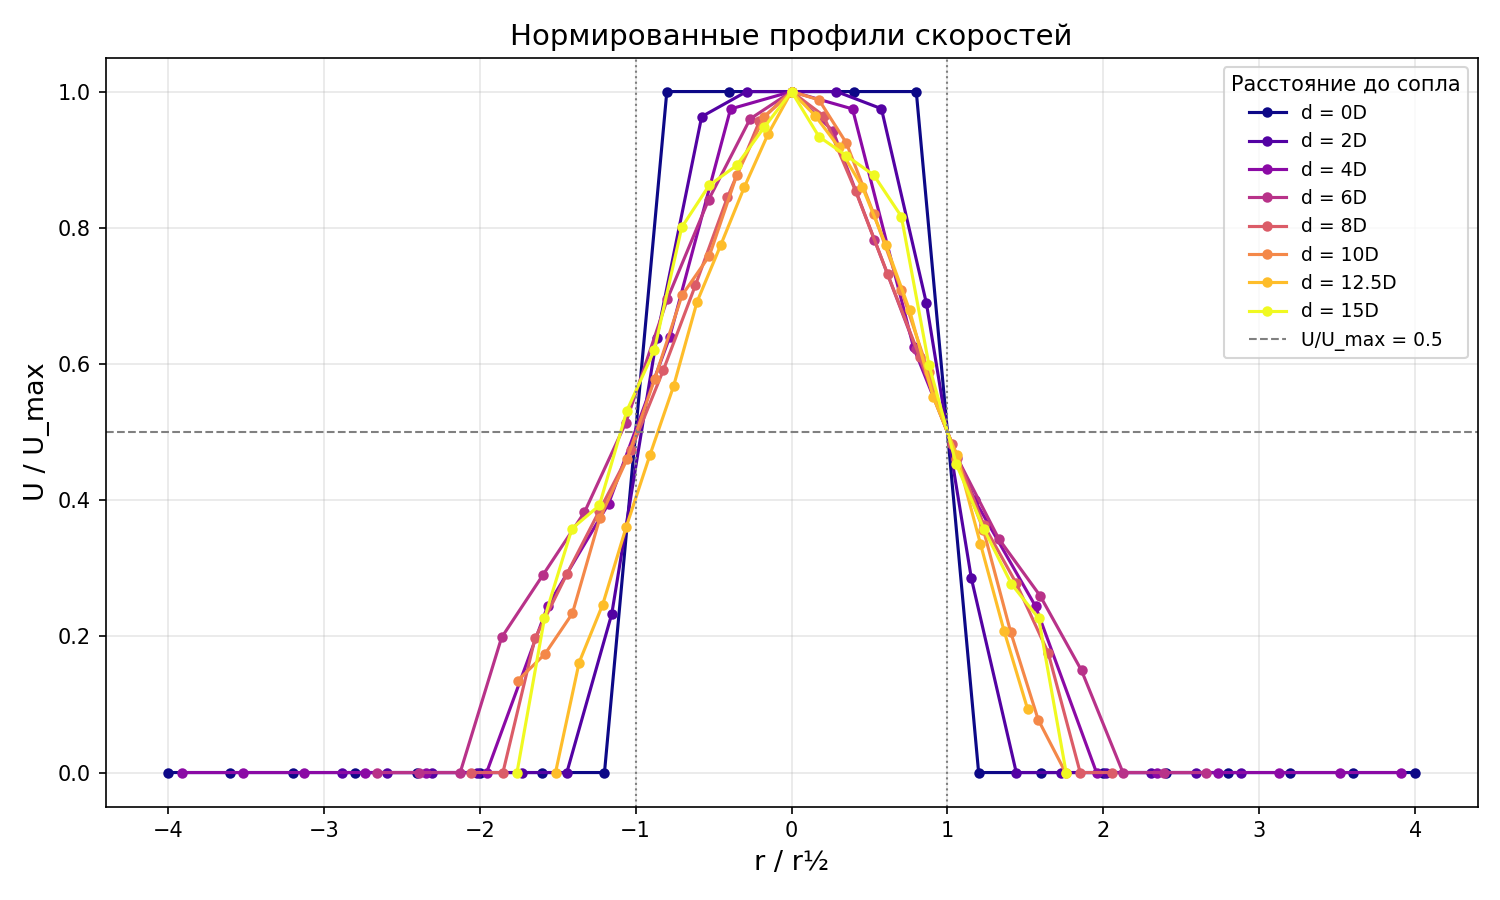
\includegraphics[width=0.75\textwidth]{photoes/velocity_normalized.png}
\caption{Нормированные профили скорости в различных сечениях}
\label{fig:velocity_profile}
\end{figure}

\begin{figure}[h!]
\centering
 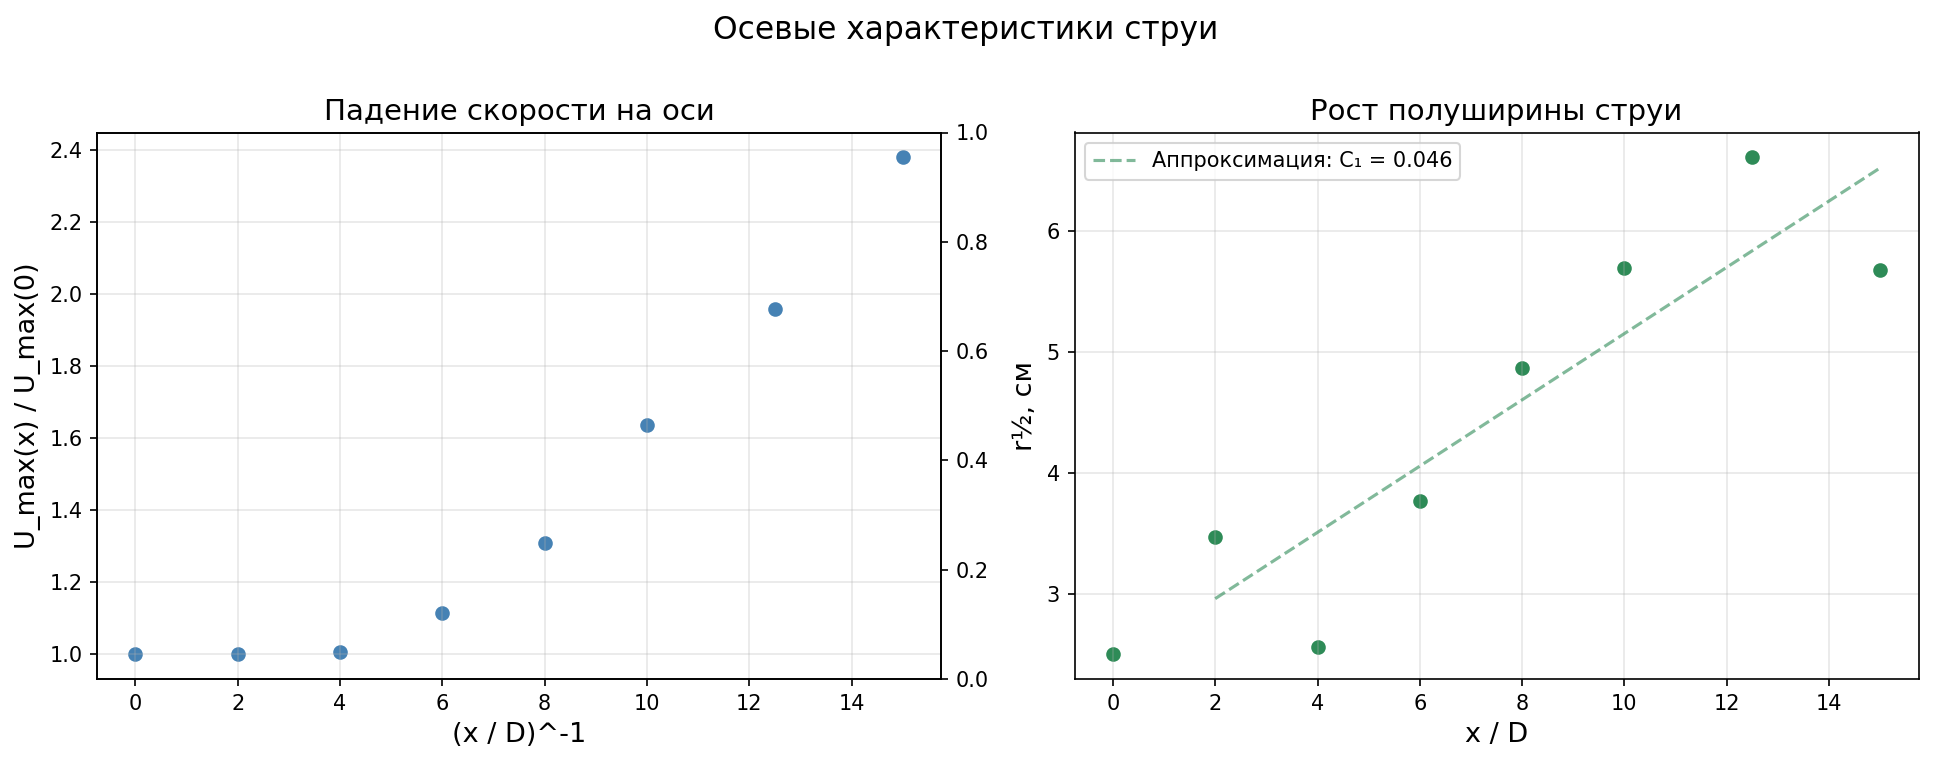
\includegraphics[width=0.8\textwidth]{photoes/characteristics.png}
\caption{Зависимости осевой скорости $U_{\text{ось}}(x)$ и полуширины $r_{1/2}(x)$}
\label{fig:characteristics}
\end{figure}

\newpage

\section{Вывод}

\begin{enumerate}
    \item Число Рейнольдса: $\ReNum = 2.3 \times 10^5 \gg 2300$, течение турбулентное от среза сопла.
    
    \item Экспериментально подтвердили наличие трёх зон струи: потенциальное ядро ($0-3D$), переходная зона ($4-6D$), основной участок ($>6D$).
    
    \item Профили скорости $U(r)$: на начальном участке имеют плоскую вершину (потенциальное ядро), по мере удаления от сопла становятся гладкими и расширяются за счёт турбулентного перемешивания.
    
    \item Осевая скорость: на основном участке убывает по гиперболическому закону $U_{\text{ось}} \sim 1/x$, что согласуется с законом сохранения импульса для свободной струи.
    
    \item Полуширина струи: линейно растёт с расстоянием $r_{1/2} = C_1 x$, угол расширения $\alpha = \arctg C_1 \approx \text{const}$. Экспериментальное значение $C_1 \approx$ 0.046.
    
    \item Автомодельность: безразмерные профили $U/U_{\text{ось}}$ от $r/r_{1/2}$ для сечений основного участка визуально совпадают, что подтверждает подобие течения в дальнем поле.

\end{enumerate}

%Экспериментальные результаты качественно согласуются с теоретическими закономерностями развития свободной турбулентной струи.

%\section*{Литература}
%\begin{enumerate}
%    \item Абрамович Г.Н. и др. \textit{Теория турбулентных струй}. -- М.: Наука, 1984.
%    \item Лойцянский Л.Г. \textit{Механика жидкости и газа}. -- М.: Наука, 1970.
%    \item Методические указания к лабораторной работе №17. -- МФТИ, 2004.
%\end{enumerate}



\end{document}